\documentclass[10pt]{amsart}
\usepackage[utf8]{inputenc}
\usepackage[margin=0.50in]{geometry} 
\usepackage{indentfirst}
\usepackage{graphicx}
\usepackage{amsthm}
\usepackage{scrextend}
\usepackage{amssymb}
\usepackage{amsmath}
\usepackage{titlesec}
\DeclareGraphicsExtensions{.pdf,.png,.jpg}
\graphicspath{{images/}}

\titleformat*{\section}{\LARGE\bfseries}

\title{\LARGE M343L: Homework Set 7 Proofs}
\author{Andrew Tseng: art2589}
\begin{document}
\maketitle
\thispagestyle{empty}

\section*{\small Problem 6.1}
\textit{1: $P \bigoplus Q = Q$ } \\
\indent\textit{2: $P \bigoplus P = O$ \quad $Q \bigoplus Q = O$ } \\
\indent\textit{3: $P \bigoplus P \bigoplus P = P \quad Q \bigoplus Q \bigoplus Q = Q$ }\\

\section*{\small Problem 6.4}
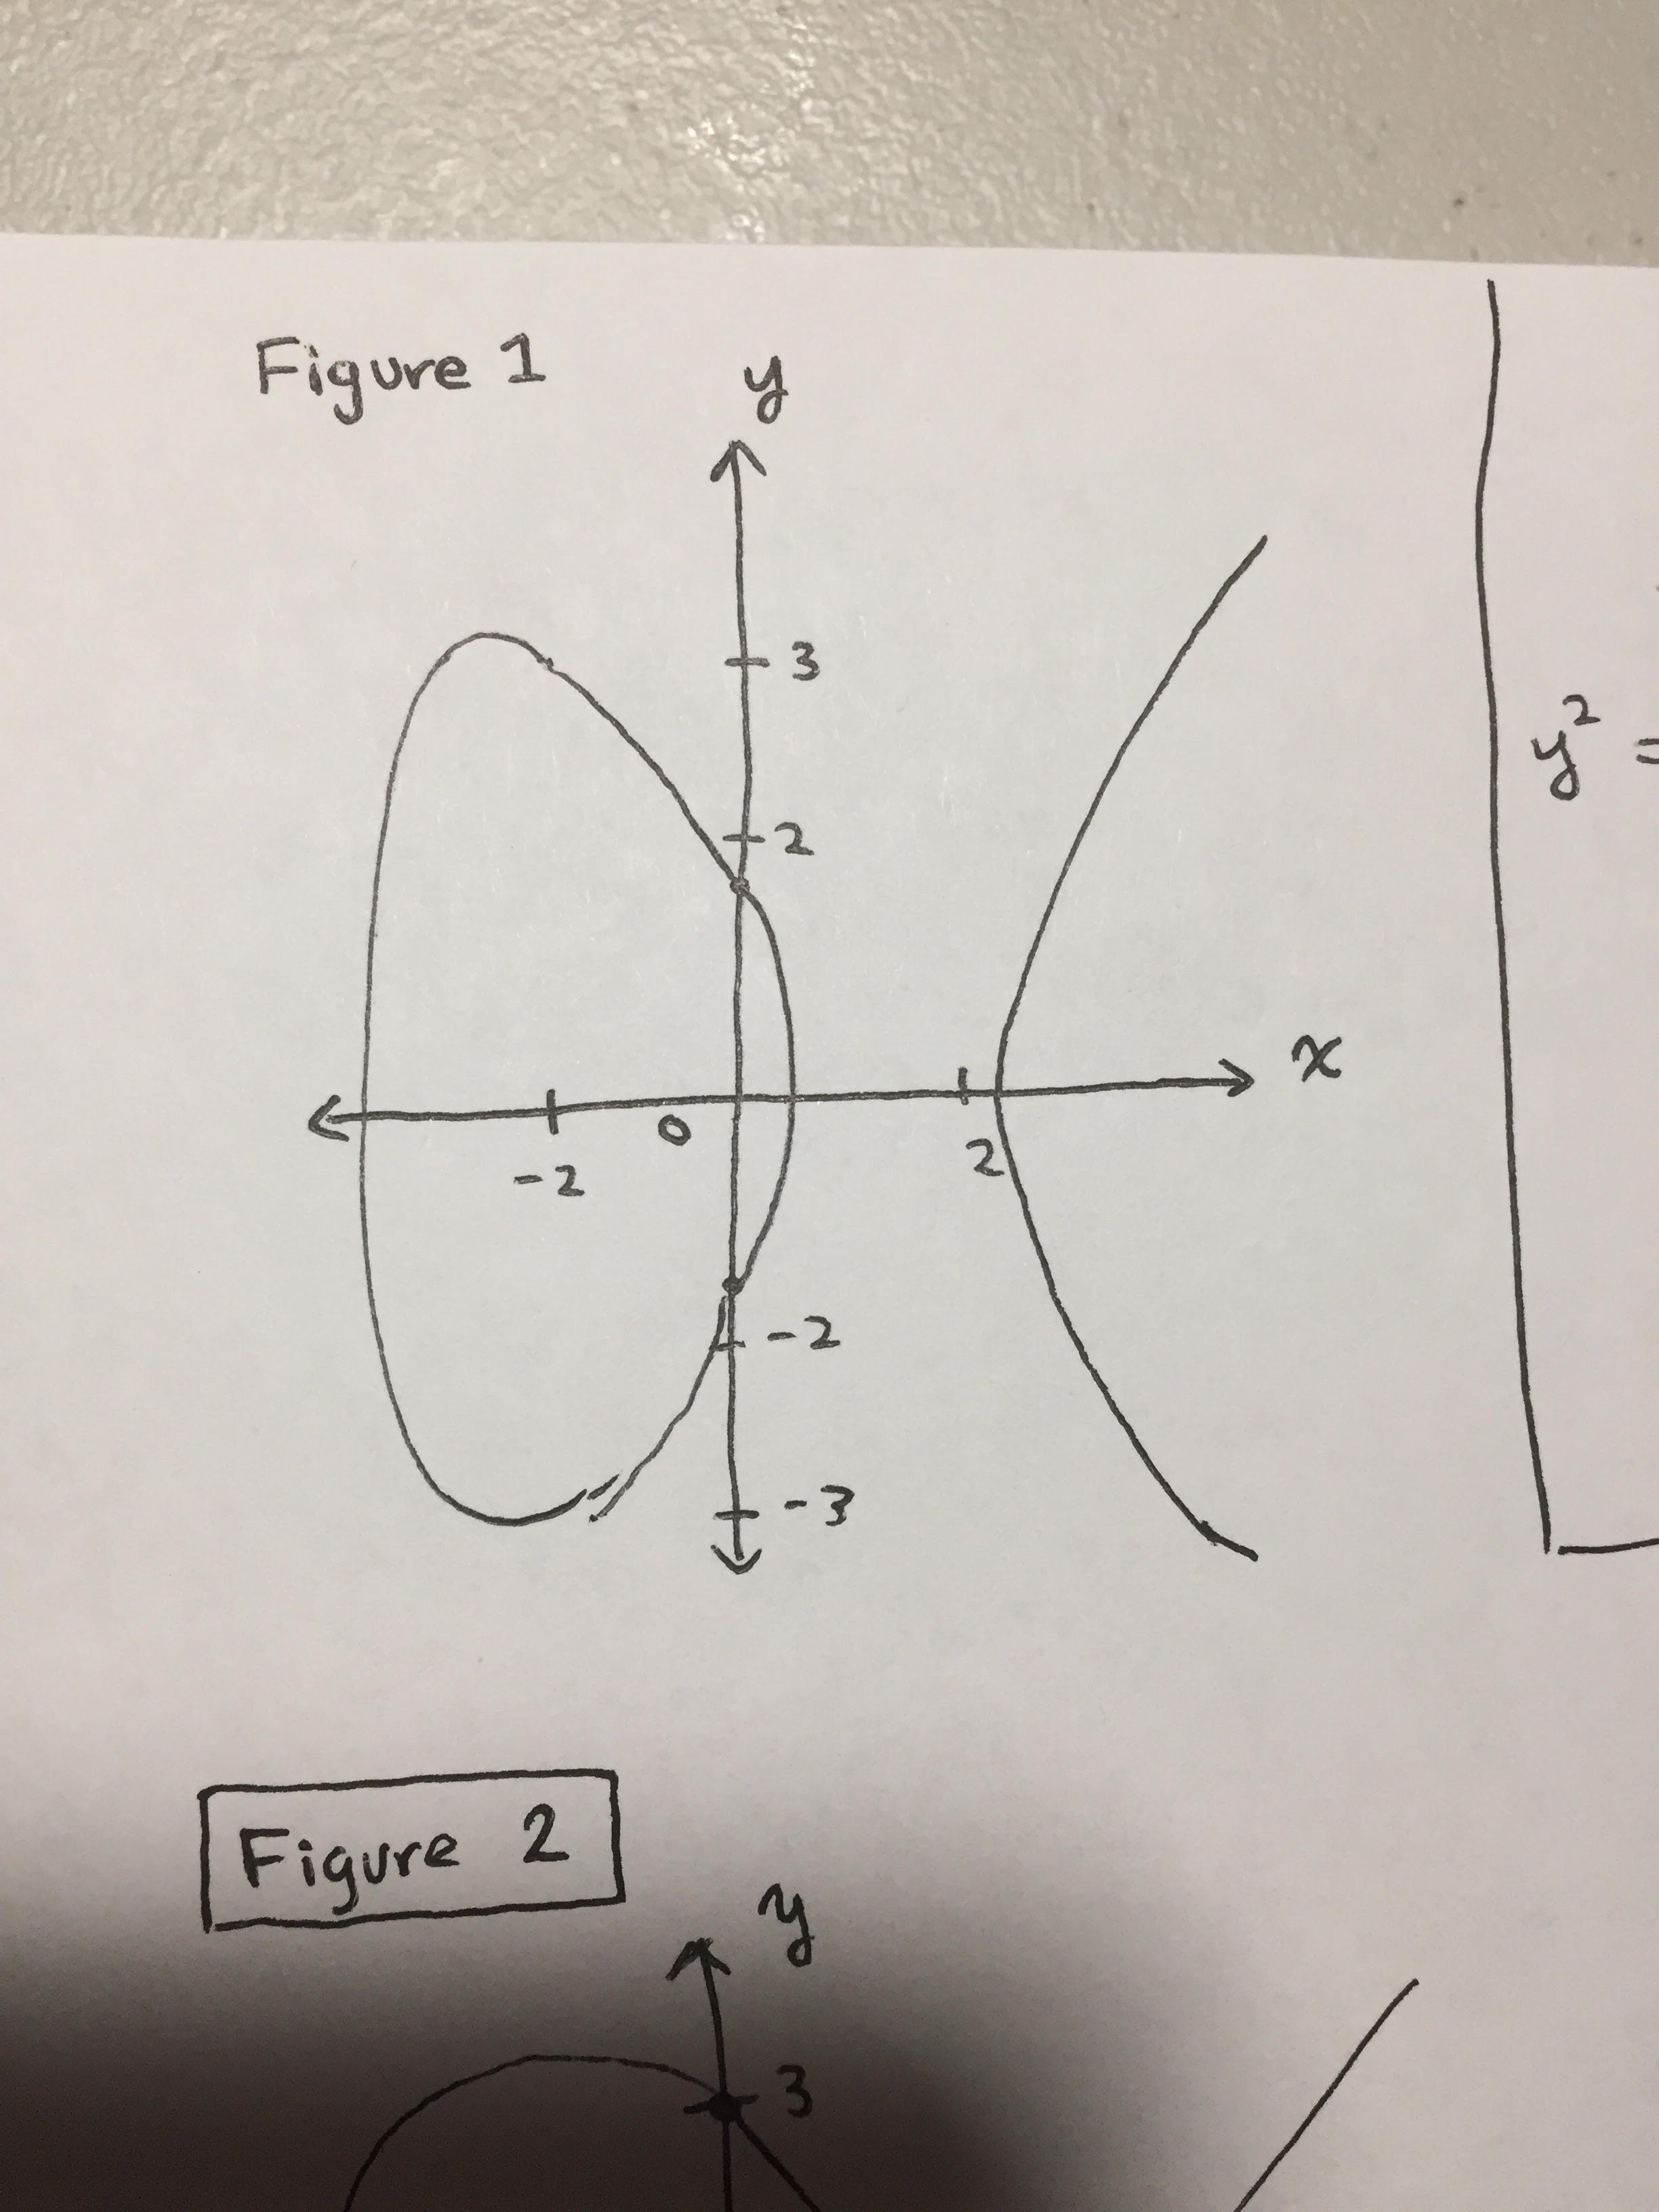
\includegraphics[scale=0.08]{graphs1}
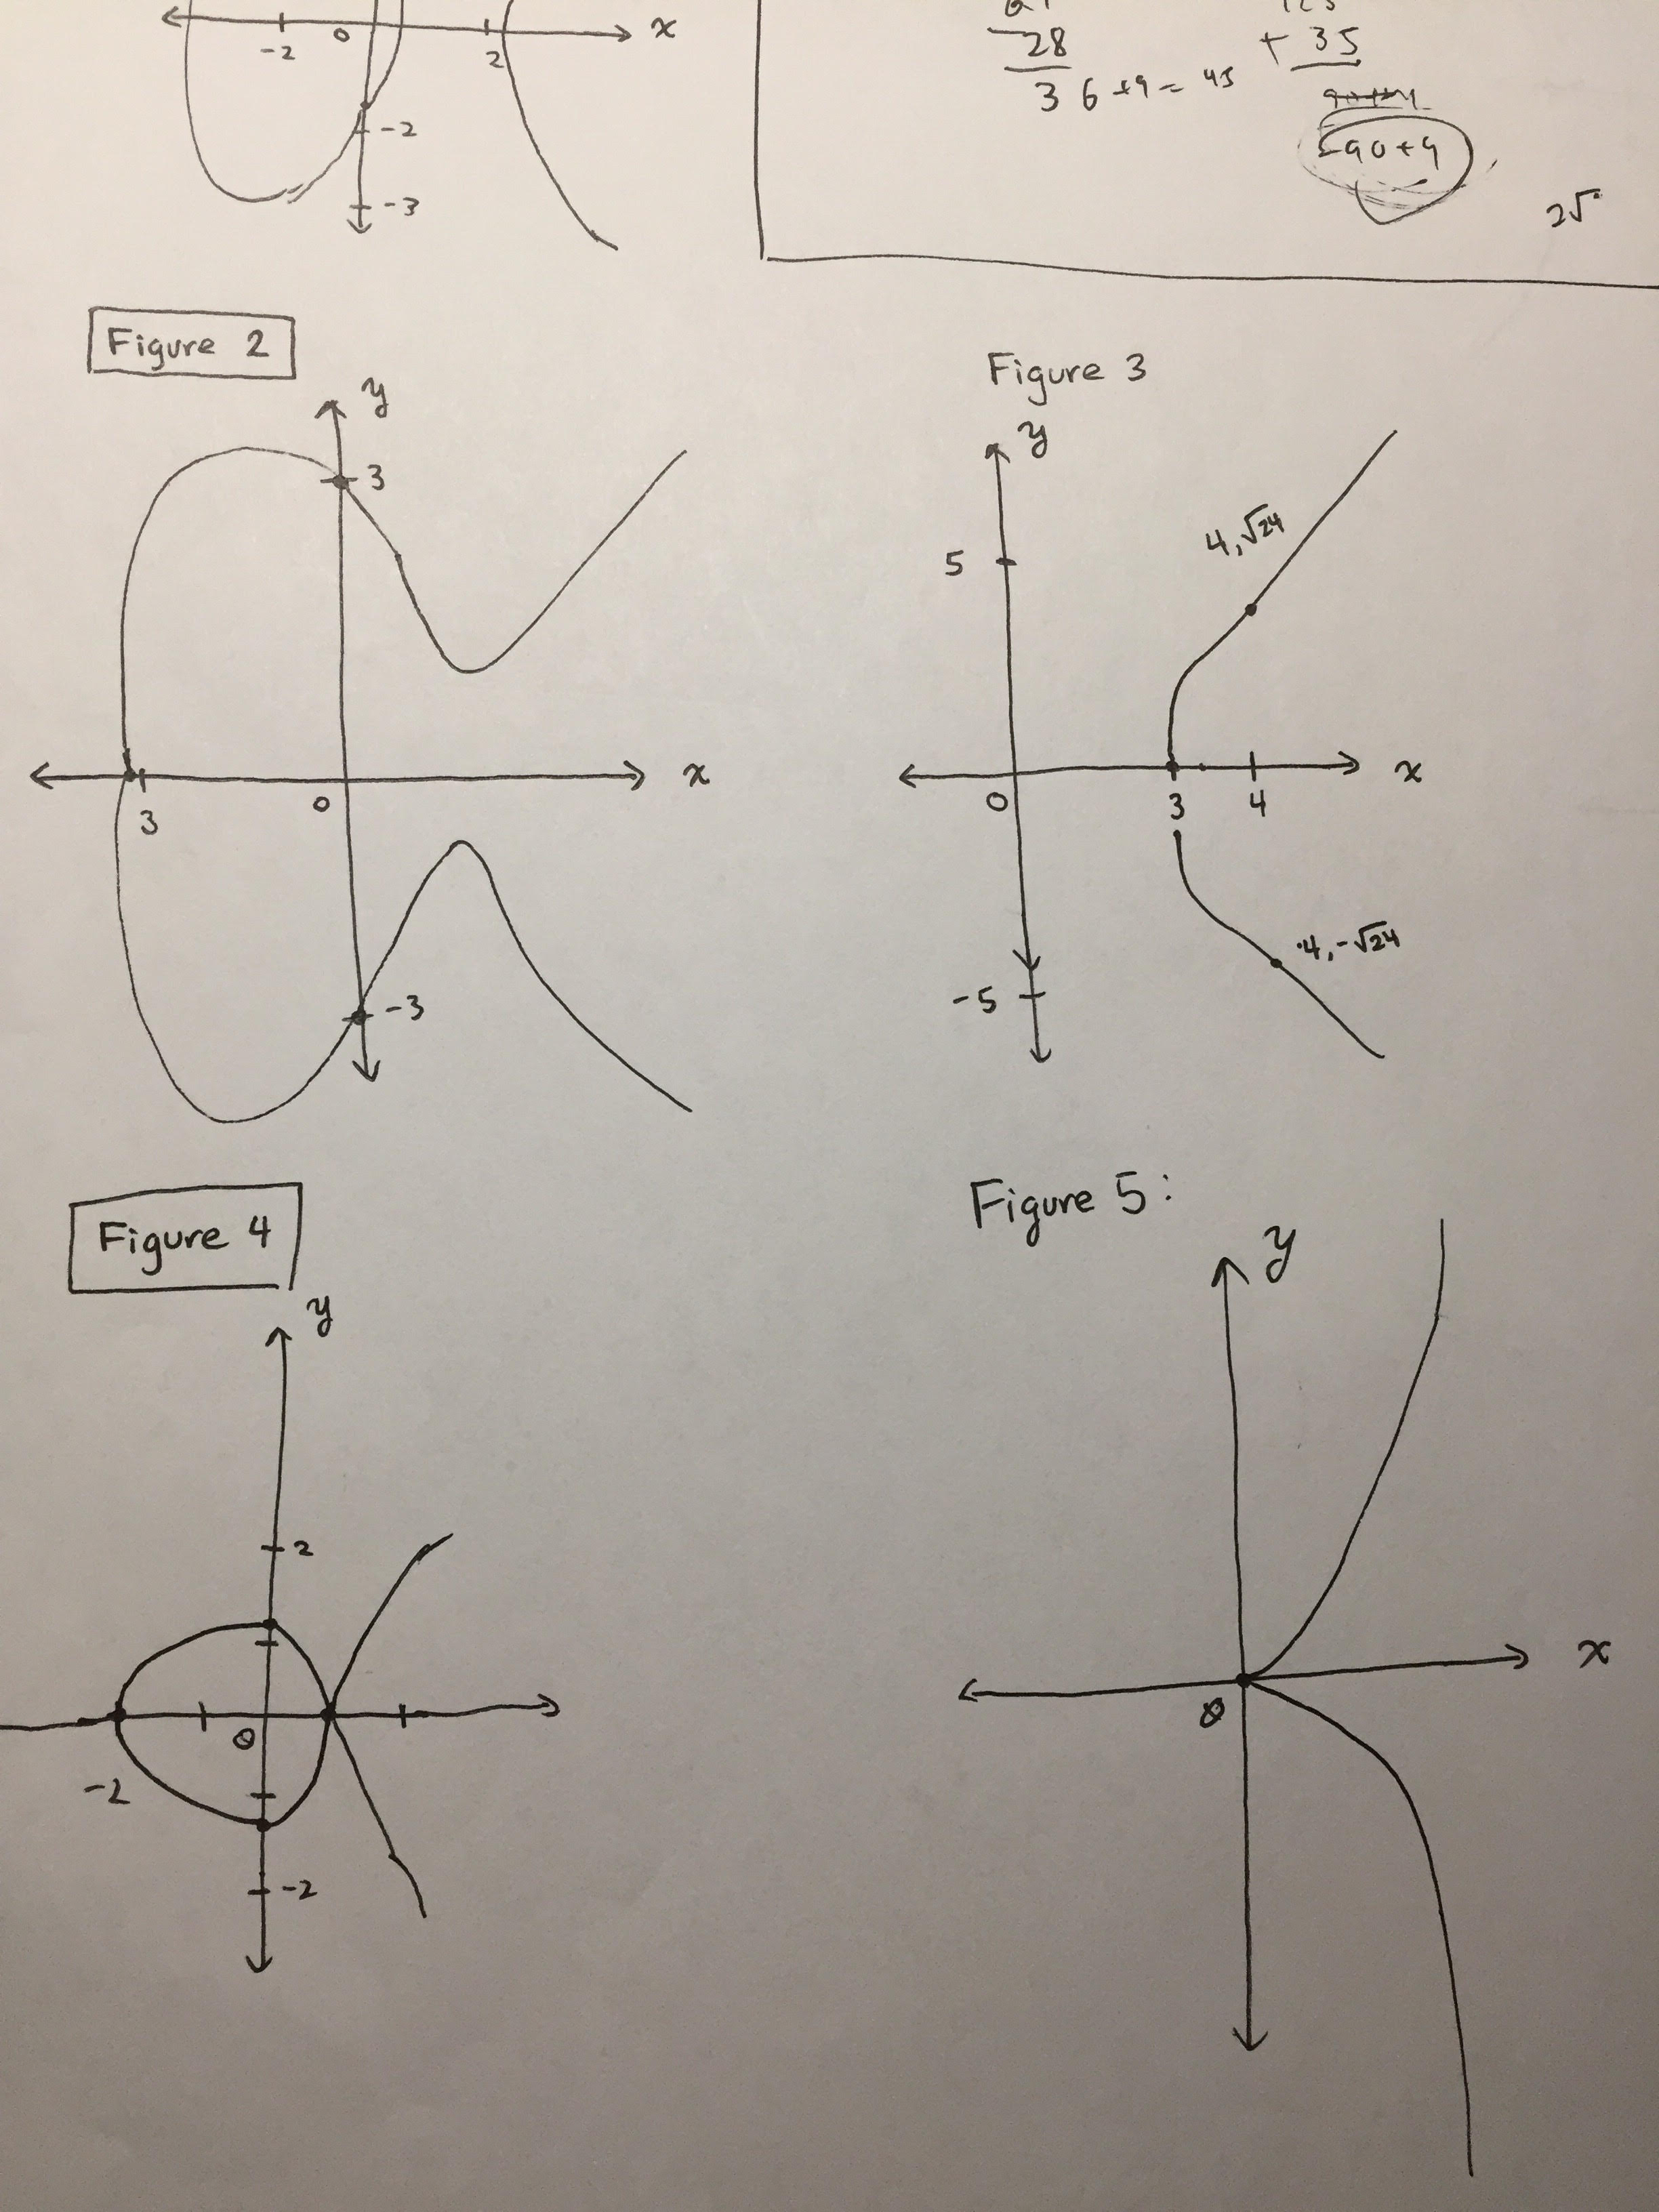
\includegraphics[scale=0.08]{graphs2} \\

\noindent Figure 4: $4(-3)^3 + 27(2)^2 = 0$, which indicates the the $\Delta E = 0$,
which indicates the the curve is not an elliptical curve. \\
Figure 5 is not an elliptical curve because $4A^3 + 27B^2 = 0$ which means all
the roots of the curve not distint (in fact they are all 0).\\

\section*{\small Problem 6.6}



\section*{\small Problem 6.10}
\small \textit{Let the point $P$ be represented by $P_{X}, P_{Y}$. $n$ is the
range of numbers from $1$ to $p$ (the field value).}
\[  \begin{bmatrix}
       P_{X}  \\
       P_{Y}  \\
    \end{bmatrix}
    \begin{bmatrix}
        n_{1} & n_{2} & ... & n_{r}\\
    \end{bmatrix}
    =
    \begin{bmatrix}
       P_{X}n_{1} & P_{X}n_{2} & ... & P_{X}n_{r} \\
       P_{Y}n_{1} & P_{Y}n_{2} & ... & P_{Y}n_{r}
    \end{bmatrix}
\]
Using the resulting matrix, you can iterate through the matrix to find a pair of
$(P_{X}n, P_{Y}n)$ that match $Q$.

\section*{\small Problem 6.13}
\small \textit{Using pollard's $\rho$ algorithm to solve ECDLP} \\
\textbf{Algorithm:} \\
\indent    step = 1 \\
\indent    while($P$ does not equal to $Q$) \\
\indent \indent        $P = P + P + P$ \\
\indent \indent        $Q = Q + Q$. \\
       \indent  step = step + 1 \\

\noindent \textbf{Example:} \\
    $P = (1,8)$,
    $Q = (12,11)$ \\
    At step 1: $P = (1,8), Q = (12,11)$. \\
    At step 2: $P = (9,6), Q = (1,5)$. \\
    At step 3: $P = (12,2), Q = (9,6)$. \\
    At step 4: $P = (2,10), Q = (2,10)$. \\
\noindent \textbf{At Step 4} $P$ equals to $Q$, thus $n = 4$ for the ECDLP.
\end{document}

